\chapter[ಅಧ್ಯಾಯ 11]{}\label{chap11}

\begin{center}
\rule{5cm}{1pt}\\[5pt]
{\Large\bfseries ಸಮಸ್ಯೆಗಳು}\\[3pt]
\rule{5cm}{1pt}
\end{center}

\begin{enumerate}
\renewcommand{\labelenumi}{\bf\theenumi.}
\itemsep=5pt
\item 6 5 7 4 3 = 26 ಅಂಕಿಗಳ ನಡುವೆ $+$, $-$, $\times$ ಬಳಸಿ ಸಮೀಕರಣ ಸರಿದೂಗಿಸಿ ಅಂಕಿಗಳ ಕ್ರಮ ಬದಲಿಸುವಂತಿಲ್ಲ. $\neq$ ನಿಷಿದ್ಧ. ಅಂಕಿಗಳ ನಡುವೆ ಒಂದು ಚಿಹ್ನೆ ಇರಲೇಬೇಕು. 

\item ಎರಡು 3 ಬಳಸಿ 20 ಬರಿಸಿ. ಗಣಿತದ ಯಾವುದೇ ಪ್ರಕ್ರಿಯೆ ಬಳಸಬಹುದು. 

\item 7 ಏಳು ಬಳಸಿ 100 ಬರಿಸಿ. ಯಾವುದೇ ಗಣಿತ ಪ್ರಕ್ರಿಯೆ ಬಳಸಬಹುದು. 

\item ಮೂರು 5 ಬಳಸಿ 60 ಬರಿಸಿ. ಯಾವುದೇ ಗಣಿತ ಪ್ರಕ್ರಿಯೆ ಬಳಸಬಹುದು. 

\item 1 2 3 4 ಈ ಅಂಕಿಗಳ ನಡುವೆ ಯಾವುದೇ ಗಣಿತ ಚಿಹ್ನೆ ಹಾಕಿ ಈ ಕೆಳಗಿನ ಸಮೀಕರಣಗಳನ್ನು ಸರಿದೂಗಿಸಿ. ಅಂಕಿಗಳ ಕ್ರಮ ಬದಲಿಸುವಂತಿಲ್ಲ. $\neq$ ನಿಷಿದ್ಧ 
\begin{tabular}[t]{lllllll}
(a) & 1 & 2 & 3 & 4 & = & 0 \\
(b) & 1 & 2 & 3 & 4 & = & 8\\
(c) & 1 & 2 & 3 & 4 & = & 24\\
(d) & 1 & 2 & 3 & 4 & = & 25
\end{tabular}

\item ಒಂದು ಗೆರೆ ಸ್ಥಾನ ಪಲ್ಲಟಮಾಡಿ, ಈ ಸಮೀಕರಣಗಳನ್ನು ಸರಿದೂಗಿಸಿ. $\neq$ ಬರು\break ವಂತಿಲ್ಲ. 

\begin{tabular}{l@{\;\;}l@{\;\;}l@{\;\;}l@{\;\;}}
(a) & VIII - I = VIII & (b) & VIII - II = IX\\
(c) & VIII - VII = XIV & (d) & VIII - III = X
\end{tabular}

\item 16 ಬೆಂಕಿಕಡ್ಡಿ ಜೋಡಿಸಿ ಈ ಆಕೃತಿ ಬರಿಸಿದೆ. ಯಾವುದಾದರೂ 2 ಕಡ್ಡಿ ಸ್ಥಾನ ಪಲ್ಲಟ ಮಾಡಿ 4 ಚೌಕ ಬರಿಸಿ. 
\begin{figure}[H]
\centering
\includegraphics[scale=1.1]{images/chap11/q7.eps}
\end{figure}

\item 24 ಬೆಂಕಿಕಡ್ಡಿ ಬಳಸಿ ಒಂದು ಚೌಕ ರಚಿಸಿದೆ. 
\begin{figure}[H]
\centering
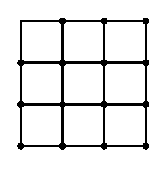
\includegraphics[scale=1.1]{images/chap11/q8.eps}
\end{figure}

\begin{itemize}
\item[(a)] 8 ಕಡ್ಡಿ ತೆಗೆದು ಹಾಕಿ 4 ಚೌಕ ಬರಿಸಿ. (ಒಂದೇ ಅಳತೆಯವು. 2 ಉತ್ತರಗಳಿವೆ.)
\item[(b)] 8 ಕಡ್ಡಿ ತೆಗೆದು ಹಾಕಿ 4 ಬೇರೆ ಬೇರೆ ಅಳತೆಯ ಚೌಕ ಬರಿಸಿ. 
\item[(c)] 6 ಕಡ್ಡಿ ತೆಗೆದು ಹಾಕಿ 6 ಚೌಕ ಬರಿಸಿ. 
\item[(d)] 8 ಕಡ್ಡಿ ತೆಗೆದು ಹಾಕಿ 5 ಚೌಕ ಬರಿಸಿ. (2 ಉತ್ತರಗಳಿವೆ.)
\end{itemize}

\item ಈ ಗುಣಾಕಾರ ಗಮನಿಸಿ. ಮುಂದಿನ 4 ಹಂತ ಬರೆಯಿರಿ. 

\begin{tabular}[t]{r@{\;}c@{\;}l}
$9\times 9 + 7$ & = & $88$\\
$9\times 98 + 6$ & = & $888$\\
$9\times 987 + 5$ & = & $8888$
\end{tabular}

\item 1 ರಿಂದ 9 ವರೆಗೆ ಎಲ್ಲ ಅಂಕಿಗಳೂ ಒಮ್ಮೆ ಮಾತ್ರ ಬರುವಂತೆ ಗುಣಾಕಾರ ರಚಿಸಿ. 

ಉದಾ: $157\times 28 = 4396$

\item ಈ ಗುಣಾಕಾರಗಳನ್ನು ಗಮನಿಸಿ. 

\begin{equation*}
\left.
\begin{aligned}
312\times 221 = 68952\\
213\times 122 = 25986  
\end{aligned}
\right\}
\begin{aligned}
& \text{ಸಂಖ್ಯೆಗಳಲ್ಲಿ ತಿರುವು ಮುರುವು}\\[-4.5pt]
& \text{ಮಾಡಿದಾಗ ಲಬ್ಧವೂ}\\[-4.5pt]
& \text{ತಿರುವು ಮುರುವು.}
\end{aligned}
\end{equation*}

\item ಈ ಗುಣಾಕಾರ ಗಮನಿಸಿ. $\underline{12}\times \underline{42} = 504 = \underline{21}\times \underline{42}$ ಗುಣಾಕಾರದ\break ಸಂಖ್ಯೆಗಳನ್ನು ತಿರುವು ಮುರುವು ಮಾಡಿದಾಗಲೂ ಅದೇ ಗುಣಲಬ್ಧ ಇಂತಹ 4 ಉದಾಹರಣೆ ರಚಿಸಿ. 

\item ಈ ಗುಣಾಕಾರ ಗಮನಿಸಿ. 

\begin{tabular}[t]{r@{\;}c@{\;}r@{\;}c@{\;}rr}
$93$ & $\times$ & $94$ & = & $87$ & $42$\\
$993$ & $\times$ & $994$ & = & $987$ & $042$\\
$9993$ & $\times$ & $9994$ & = & $9987$ & $0042$\\
\end{tabular}

\vskip 0.2cm

ಮುಂದಿನ ಮೂರು ಹಂತ ಬರೆಯಿರಿ. 

\item ಈ ಆಕೃತಿಯನ್ನು 4 ಸರ್ವ ಸಮ ಭಾಗಗಳಾಗಿ ಕತ್ತರಿಸಿ. 
\begin{figure}[H]
\centering
\includegraphics[scale=1.3]{images/chap11/q14.eps}
\end{figure}

\item 5 ಚೌಕಗಳನ್ನು ಪರಸ್ಪರ ಲಗತ್ತಿಸಿರುವಂತೆ ಎಷ್ಟು ರೀತಿ ಜೋಡಿಸಬಹುದು? (12 ಬಗೆ ಇದೆ. ಅವನ್ನು ರಚಿಸಿ) ಅವುಗಳಲ್ಲಿ ಯಾವ 2ನ್ನು ಲಗತ್ತಿಸಿರುವಂತೆ ಜೋಡಿಸಿ ಈ ಆಕೃತಿ ಬರಿಸಬಹುದು? 
\begin{figure}[H]
\centering
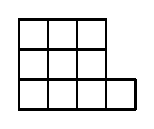
\includegraphics[scale=1.4]{images/chap11/q15.eps}
\end{figure}

\item ಒಂದು ಚೌಕದೊಳಗೆ ಬೇರೆ ಬೇರೆ ಅಳತೆಯ ಸಮದ್ವಿ ಬಾಹು ಲಂಬಕೋನ ತ್ರಿಭುಜಗಳನ್ನು ರಚಿಸಿ. ಅತಿ ಕಡಿಮೆ ತ್ರಿಭುಜಗಳನ್ನು ಬಳಸಿ. (2 ಉತ್ತರದಗಳುವೆ.)

\item 16 ಬಿಂದುಗಳನ್ನು 4 $\times$ 4 ಹಂದರದಲ್ಲಿ ಸಮಾನ ದೂರದಲ್ಲಿರುವಂತೆ ಜೋಡಿಸಿದೆ. ಎಲ್ಲ ಬಿಂದುಗಳ ಮೂಲಕ ಹೋಗುವಂತೆ, ಪೆನ್ಸಿಲ್ ಎತ್ತದೆ, ಹಿಮ್ಮುಖ ಚಲಿಸದೆ, ಹೋದಗೆರೆಯಲ್ಲೇ ಹೋಗದೆ ಚಲಿಸುವಂತೆ ರೇಖೆ ಎಳೆಯಿರಿ. 
\begin{figure}[H]
\centering
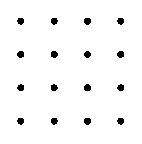
\includegraphics[scale=1.2]{images/chap11/q17.eps}
\end{figure}


\item ಶ್ರುತ್ವಾ ವರ್ಷಾಭ್ರ ಮಾಲಾಪಟಹ ಪಟುರವಂ ಶೈಲ ಶೃಂಗೇರು ರಂಗೇ ।

ನಾಟ್ಯಂ ಚಕ್ರೇ ಪ್ರಮೋದ ಪ್ರಮುದಿತ ಶಿಖಿನಾಂ ಷೋಡಶಾಂಶೋಏಷ್ಟಮಾಶ್ಯ ।।

ತ್ರ್ಯಂಶಃ ಶೇಷಸ್ಯಷಷ್ಠೋತರ ಬಕುಲವನೇ ಪಂಚಮೂಲಾನಿತಸ್ಥುಃ ।

ಪುನ್ನಾಗೇ ಪಂಚ ದೃಷ್ಟಾ ಬಭಣಗಣಕಗಣಂ ಬರ್ಹಿಣಾಂಸಂಗುಣಯ್ಯ 

\smallskip

\hfill \{ವರಾಹಮಿಹಿರಾಚಾರ್ಯಕ `ಗಣಿತ ಸಾರ ಸಂಗ್ರಹ'ದಿಂದ\}

\smallskip

{\bf ಅರ್ಥ:} ವರ್ಷ ಋತುವಿನಲ್ಲಿ ಮೋಸಗಳ ಸಮೂಹದಿಂದ ಉಂಟಾದ ಸ್ಪಷ್ಠ ಧ್ವನಿಯನ್ನು ಕೇಳಿ ನವಿಲುಗಳ ಒಂದು ಸಮೂಹದ ಹದಿನಾರನೇ ಒಂದು ಭಾಗ ಮತ್ತು ಎಂಟನೇ ಒಂದು ಭಾಗಗಳಷ್ಟು ಮತ್ತು ಉಳಿದುದ ಮೂರನೆ ಒಂದು ಭಾಗ ಹಾಗೂ ಅನಂತರ ಉಳಿದುದರ ಆರನೇ ಒಂದು ಭಾಗಗಳಷ್ಟು ನವಿಲುಗಳು ಆ ನಂದಾ ತಿರೇಖದಿಂದ ಪರ್ವತ ಶಿಕರವೇಮ್ಬ ವಿಶಾಲವಾದ ನಾಟ್ಯ ಶಾಲೆಯಲ್ಲಿ ನರ್ತಿಸಲಾರಂಭಿಸಿದುವು. ಸಮೂಹದ ವರ್ಗ ಮೂಲದ ಐದರಷ್ಟು ನವಿಲುಗಳು ಬಕುಲ ವೃಕ್ಷಗಳ ಉತ್ಕೃಷ್ಟವಾದ ಕಾಡಿನಲ್ಲಿ ವಿಹರಿಸುತ್ತಿದ್ದುವು. ಇನ್ನು ಉಳಿದ 5 ನವಿಲುಗಳು ಪುನ್ನಾಗ ವೃಕ್ಷದ ಮೇಲೆ ಕಾಹಿಲ್ಪಟ್ಟುವು. ಎಲೈ ಗಣಿತಜ್ಞನೇ, ಲೆಕ್ಕ ಮಾಡಿ ಆ ಸಮೂಹದಲ್ಲಿ ಎಷ್ಟು ನವಿಲುಗಳು ಇದ್ದುವು ಎಂಬುದನ್ನು ಹೇಳು.  

\item ಮಹಿಷೀಹಾಂ ಅಷ್ಟಾಂಶವ್ಯೋಕೋ ವರ್ಗೀಕೃತೋ ವನೇರಮತೇ ।

ಪಂಚದಶಾದ್ರೌ ದೃಷ್ಟಾ ಸ್ತೃಣಂ ಚರಂತ್ಯಃ ಕಿಯಂತ್ಯಸ್ತಾಃ ।।

\smallskip

\hfill (ವರಾಹಮಿರಾಚಾರ್ಯರ `ಗಣಿತಸಾರ ಸಂಗ್ರಹ'ದಿಂದ)

\smallskip

{\bf ಅರ್ಥ:} ಎಮ್ಮೆಗಳ ಒಂದು ಗುಂಪಿನ ಎಂಟನೇ ಒಂದು ಭಾಗದಿಮ್ದ ಒಂದು ಕಡಿಮೆ ಮಾಡಿ ಅದರ ವರ್ಗದಷ್ಟು ಎಮ್ಮೆಗಳು ಕಾಡಿನಲ್ಲಿ ರಮಿಸುತ್ತಿದ್ದುವು. ಉಳಿದ 15 ಗುಡ್ಡದ ಮೇಲೆ ಹುಲ್ಲನ್ನು ಮೇಯುತ್ತಿದ್ದಂತೆ ಕಂಡುವು. ಒಟ್ಟು ಇದ್ದ ಎಮ್ಮೆಗಳೆಷ್ಟು? 

\item ಒಂದು ಸೀಸದ ಗೋಳ (sphere)ವನ್ನು ಕರಗಿಸಿ ಸಣ್ಣಗೋಳಗಳನ್ನಾಗಿ ಮಾಡಿದೆ. ಸಣ್ಣಗೋಳಗಳ ತ್ರಿಜ್ಯ ದೊಡ್ಡಗೋಳದ ತ್ರಿಜ್ಯದ ಅರ್ಧದಷ್ಟಿದೆ. ಎಷ್ಟು ಸಣ್ಣಗೋಳಗಳಾಗುತ್ತವೆ? 

\item ಒಂದು ಆಯತಾಕಾರದ ಲೋಹದ ಘನದ ಅಳತೆಗಳು 49 cm, 44 cm ಮತ್ತು 18 cm. ಇದನ್ನು ಕರಗಿಸಿ ಒಂದು ಗೋಳವನ್ನಾಗಿ ಎರಕಹೊಯ್ದಿದೆ. ಗೋಳದ ತ್ರಿಜ್ಯವೆಷ್ಟು? 

\item 
\begin{tabular}[t]{r}
REAP\\
REAP\\
REAP\\
\hline
HEAPS
\end{tabular}

ಇದು ಅಕ್ಷರ ಸಂಕಲನ ಲೆಕ್ಕ (alpha magic) 0, 4 ಬಳಸಿಲ್ಲ ಪರಿಹರಿಸಿ. 

\item ಒಬ್ಬನಲ್ಲಿ 3ಲೀ, 5ಲೀ ಅಳತೆ ಪಾತ್ರೆಗಳಿವೆ. ನಿರಿನ ತೊಟ್ಟಿಯಿಂದ ಸರಿಯಾಗಿ 4ಲೀ ನೀರು ತರಬೇಕು. ಬೇರೆ ಯಾವ ಪಾತ್ರೆ ಬಳಸುವಂತಿಲ್ಲ ಹೇಗೆ?  

\item ಗಾಂಪರ ಲೆಕ್ಕ : ಒಮ್ಮೆ ಗಾಂಪ ಮಠದ ಶಿಷ್ಯರಾದ ಮಂಕ, ಮಹೆಯ, ಮಡ್ಡಿ, ಮೂರ್ಖ, ಮುಟ್ಠಾಳ, ಮುಸುರ, ಮಂಕುದಿಣ್ಣೆ  - ಏಳು ಜನರೂ ಬೆಂಗಳೂರು ನೋಡಲು ಹೊರತರು. ಗುರುಗಳು ಅನುಮತಿಸಿ ಒಬ್ಬೊಬ್ಬರಿಗೂ 50ರೂ ಕೊಟ್ಟು ಜಾಗ್ರತೆಯಿಂದ ಹೋಗಿ ಬನ್ನಿ ಎಂದು ಆಶೀರ್ವದಿಸಿದರು. 

\vskip 0.2cm

7 ಜನರೂ ಬಸ್ಸಿನಲ್ಲಿ ಬೆಂಗಳೂರಿನ ಮೆಜೆಸ್ಟಿಕ್ ತಲುಪಿದರು. ವಿಧಾನಸೌಧ ನೋಡಬೇಕೆಂದು ಆಟೊವನ್ನು ಹಿಡಿದರು. ರಿಕ್ಷಾ ಚಾಲಕ ``7 ಜನರಿದ್ದೀರಿ ಸ್ವಲ್ಪ ಹೆಚ್ಚಿಗೆ ಬಾಡಿಗೆ ಕೊಡಬೇಕು ಎಂದ ಒಪ್ಪಿದರು. ವಿಧಾನಸೌಧಕ್ಕೆ ಬಂದರು. ರಿಕ್ಷಾ ಮೀಟರ್ 28ರೂ ಆಗಿತ್ತು. ಚಾಲಕ ಹೆಳಿದ ``ಪ್ರತಿಯೊಬ್ಬರೂ 13ರೂ ಕೊಡಬೇಕು". ಎಲ್ಲರೂ ದುಡ್ಡು ತೆಗೆಯಲು ಜೇಬಿಗೆ ಕೈ ಹಾಕಿದರು. ಮಂಕ ಹೇಳಿದ. ತಡೆಯಿರಿ. ನಾನು ಭಾಗಾಕಾರದಲ್ಲಿ ನಿಪುಣ. ಚಾಲಕನ ಲೆಕ್ಕ ಸರಿ ಇದೆಯೇ ನೋಡುತ್ತೇನೆ. ಕಾಗದ, ಪೆನ್ನು ತೆಗೆದು ಲೆಕ್ಕ ಹಾಕಿದ ಸರಿಯಾಗಿದೆ ಚಾಲಕನ ಲೆಕ್ಕ ಎಂದ. ಎಲ್ಲರೂ ಮತ್ತೆ ಜೋಬಿಗೆ  ಕೈ ಹಾಕಿದರು. 

\begin{tabular}[t]{l@{\;}r@{\;}l}
7)& 28& (13\\
& 7 & \\
\hline
& 21& \\
& 21 &\\
\hline
\end{tabular}

ಅಷ್ಟರಲ್ಲಿ ಮಡೆಯ ಹೇಳಿದ. ತಡೆಯಿರಿ. ನಾನು ಗುಣಾಕಾರದಲ್ಲಿ ಪರಿಣಿತ ಲೆಕ್ಕಿಸಿ ಹೇಳುತ್ತೇನೆ. ಕಾಗದ, ಪೆನ್ನು ಬಳಸಿ ಲೆಕ್ಕಿಸಿದ. 

\begin{tabular}[t]{c}
13$\times$ 7\\
\hline
21\\
7\\
\hline
28\\
\hline
\end{tabular}

ಸರಿಯಾಗಿದೆ. ಚಾಲಕನ ಲೆಕ್ಕ ಎಂದ. ಮತ್ತೆ ಎಲ್ಲರ ಕೈ ಜೋಬಿಗೆ. ಅಷ್ಟರಲ್ಲಿ ಮಡ್ಡಿ ಹೇಳಿದೆ. ``ತಡೆಯಿರಿ ನಾನು ಕೂಡುವ ಲೆಕ್ಕದಲ್ಲಿ ಬುದ್ಧಿವಂತ. ಲೆಕ್ಕಿಸಿ ಹೇಳುತ್ತೇನೆ". ಕಾಗದ, ಪೆನ್ನು ತೆಗೆದುಕೊಂಡು ಲೆಕ್ಕಿಸಿದ. 

\begin{tabular}[t]{c}
13\\
13\\
13\\
13\\
13\\
13\\
13\\
\hline
28\\
\hline
\end{tabular} 

\smallskip

ಬಿಡಿಸಾಲಿನ 3ಗಳನ್ನು ಕೂಡಿಸಿದ. 21 ಬಂದಿರು. ಅದಕ್ಕೆ ಹತ್ತಿರ ಸಾಲಿನ 1ಗಳನ್ನು ಕುಡಿಸಿದ. 28 ಬಂತು. ಚಾಲಕನ ಲೆಕ್ಕ ಸರಿ ಇದೆ ಎಂದ. 

ಪ್ರತಿಯೊಬ್ಬರೂ 13ರೂನಂತೆ ಕೊಟ್ಟರು. ಹೇಗಿದೆ ಗಾಂಪರ ಲೆಕ್ಕ. 

\item ಒಬ್ಬನಲ್ಲಿ 2 ದಾರದ ತುಮ್ಡುಗಳಿದ್ದುವು. ಒಂದು ಇನ್ನೊಂದರ ಎರಡರಷ್ಟಿದ್ದರು. ಪ್ರತಿ ತುಂಡಿನಲ್ಲಿಯೂ 6 ಅಂಗುಲ ಉದ್ದದ ದಾರ ಕತ್ತರಿಸಿದ. ಉಳಿದ ತುಂಡುಗಳು ಒಂದು ಇನ್ನೊಂದರ ಮೂರರಷ್ಟು ಉದ್ದ ಇದ್ದಿತು. ದಾರಗಳ ಮೊದಲ ಉದ್ದವೆಷ್ಟು? 

\item ಒಂದು ಸಂಖ್ಯೆಯ ವರ್ಗದ 8ರಷ್ಠಕ್ಕೆ 1 ಕುಡಿಸಿದಾಗ ಒಂದು ವರ್ಗಸಂಖ್ಯೆ ಬರುತ್ತದೆ. ಕನಿಷ್ಠ ಸಂಖ್ಯೆ ಯಾವುದು? 

\item 3 ವರ್ಷದ ನಂತರದ ನನ್ನ ವಯಸ್ಸಿನ 3 ರಷ್ಟರಿಂದ, ಈಗಿನ ವಯಸ್ಸಿನ 3 ವರ್ಷಗಳ ಹಿಂದಿನ ವಯಸ್ಸಿನ 3 ರಷ್ಟು ಕಳೆದರೆ ನನ್ನ ಈಗಿನ ವಯಸ್ಸು ಲಭಿಸುತ್ತದೆ. ಈಗಿನ ವಯಸ್ಸೆಷ್ಟು? 

\eject

\item ಈ ಸಂಖ್ಯೆಗಳ ವಿಶಿಷ್ಟತೆ ಗಮನಿಸಿ. 

\begin{tabular}[t]{r@{\;}c@{\;}l}
$153$ & = & $1^{3} + 5^{3} + 3^{3}$\\[0.1cm]
$370$ & = & $3^{3} + 7^{3} + 0^{3}$\\[0.1cm]
$371$ & = & $3^{3} + 7^{3} + 1^{3}$\\[0.1cm]
$407$ & = & $4^{3} + 0^{3} + 7^{3}$\\[0.1cm]
$4913$ & = & $(4 + 9 + 1 + 3)^{3} = 17^{3}$\\[0.1cm]
$165033$ & = & $16^{3} + 50^{3} + 33^{3}$
\end{tabular}

\item ಅಪೂರ್ವ ಪೂರ್ಣಾಂಕ ಚತುಷ್ಟಯ 1, 3, 8, 120

ಈ ಶ್ರೇಣಿಯ ಯಾವುದೇ ಎರಡು ಸಂಖ್ಯೆಗಳ ಗುಣಲಬ್ಧಕ್ಕೆ 1ನ್ನು ಕೂಡಿಸಿದರೆ ಲಭಿಸುವ ಸಂಖ್ಯೆ ಪೂರ್ಣವರ್ಗ 

\vskip 0.2cm

\begin{tabular}[t]{ll}
$1 \times 3 + 1 = 4 = 2^{2}$ & $3\times 8 + 1 = 25 = 5^{2}$\\
$1 \times 8 + 1 = 9 =32^{2}$ & $3\times 120 + 1 = 361 = 19^{2}$\\
$1 \times 120 + 1 = 121 = 11^{2}$ & $8\times 120 + 1 = 961 = 31^{2}$\\
\end{tabular}

\vskip 0.1cm

ಈ ಶ್ರೇಣಿಯಲ್ಲಿ 120 ಕ್ಕಿಂತ ದೊಡ್ಡ ಸಂಖ್ಯೆ ಇಲ್ಲ ಎಂದು ಸಾಧಿಸಲಾಗಿದೆ. 

\item ಅಪವರ್ತನಗಳ ಮೊತ್ತ ಪೂರ್ಣವರ್ಗವಾಗಿರುವಂತಹ ಸಂಖ್ಯೆಗಳು 

\begin{tabular}[t]{lllll}
 & ಸಂಖ್ಯೆ & ಅಪವರ್ತನಗಳು & ಮೊತ್ತ & \\
 (1) & $3$ & $1, 3$ & $4$ & = $2^{2}$\\
 (2) & $66$ & $1, 2, 3, 6, 11, 22, 33, 66$ & $144$ & = $12^{2}$\\
 (3) & $70$ & $1, 2, 5, 7, 10, 14, 35, 70$ & $144$ & = $12^{2}$\\
 (4) & $81$ & $1, 3, 9, 27, 81$ & $121$ & = $11^{2}$\\
 (5) & $1501$ & $1, 19, 79, 1501$ & $1600$ & = $40^{2}$
\end{tabular}
\end{enumerate}

\smallskip

\begin{center}
\rule{5cm}{1pt}\\[3pt]
{\Large\bfseries ಉತ್ತರಗಳು}\\[-0.1cm]
\rule{5cm}{1pt}
\end{center}

\begin{enumerate}
\itemsep=5pt

\item $6 - 5 + 7 \times 4 - 3 = 26$

(ಭಾಗುಕೂಕ ನಿಯಮ ಭಾಗಿಸು, ಗುಣಿಸು, ಕುಡು, ಕಳೆ ಪ್ರಕ್ರಿಯೆಗಳನ್ನು ಕ್ರಮವಾಗಿ ಮಾಡಬೇಕು. BODHAS $-$ bracket, order, Division, Multification, Addition, Subtraction)

\item $\dfrac{3!}{\cdot 3} = \dfrac{3\times 2\times 1}{\cdot 3} = \dfrac{6}{\cdot 3} = \dfrac{60}{3} = 20$

\vskip 0.3cm

\item $(7\times 7) + (7\times 7) + {(7 + 7) \div 7}$

\vskip 0.1cm

$49 + 49 + 14 \div 7 = 49 + 49 + 2 = 100$

\item  $55 + 5 = 60$

\item 
\begin{tabular}[t]{lll}
(a) & $(1 + 2 - 3)\times 4$ &  = $0$\\
(b) & $-1 + 2 + 3 + 4$ & = $8$\\
(c) & $1\times 2\times 3\times 4$ &  = $24$\\
(d) & $1 + 2\times 3\times 4$ &  = $25$\\
& (ಗುಣಿಸಿ, ಕೂಡಿ) & 
\end{tabular}

\vskip 0.3cm

\item 
\begin{itemize}
\item[(a)] VII $+$ I = VIII (VIII ನ I ನ್ನು $-$ ಮೇಲೆ ಇರಿಸಿದೆ.)
\item[(b)] VII $+$ II = IX (VIII ನ I ಗೆರೆಯನ್ನು $-$ ಮೇಲೆ ಇರಿಸಿದೆ.)
\item[(c)] VIII $+$ VI = XIV (VII ನ ಒಂದು I ಗೆರೆಯನ್ನು $-$ ಮೇಲಿಟ್ಟಿದೆ)
\item[(d)] VII $+$ III = X (VIII ನ ಒಂದು I ಗೆರೆ $-$ ಮೇಲಿರಿಸಿದೆ.)
\end{itemize}

\item ಕೊಟ್ಟಿರುವುದು 

\vskip -0.2cm

\begin{figure}[H]
\centering
\includegraphics{images/chap11/ans7.eps}

\hspace{4cm}\text{ಸ್ಥಾನ ಪಲ್ಲಟ ಮಾಡಿದೆ.}
\end{figure}

\item 
~

\begin{figure}[H]
\centering
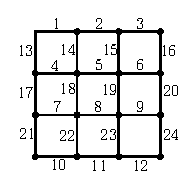
\includegraphics[scale=1.3]{images/chap11/ans8.eps}
\end{figure}


\begin{minipage}[c]{4cm}
\begin{figure}[H]
\centering
\includegraphics{images/chap11/ans8a1.eps}

\hspace{4cm}\text{1, 13, 3, 16, 21, 10, 12, 24 ತೆಗೆದಿದೆ. }
\end{figure}
\end{minipage}
\qquad
\begin{minipage}[c]{5cm}
\begin{figure}[H]
\centering
\includegraphics{images/chap11/ans8a2.eps}

\hspace{4cm}\text{2, 5, 17, 18, 19, 20, 8, 11 ತೆಗೆದಿದೆ.}
\end{figure}
\end{minipage}

\begin{minipage}[c]{4cm}
\begin{figure}[H]
\centering
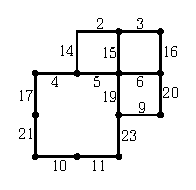
\includegraphics{images/chap11/ans8b.eps}

\hspace{4cm}\text{1, 13, 12, 26, 7, 8, 18, 22 ತೆಗೆದಿದೆ.}
\end{figure}
\end{minipage}
\qquad
\begin{minipage}[c]{5cm}
\begin{figure}[H]
\centering
\includegraphics{images/chap11/ans8c.eps}

\hspace{4cm}\text{2, 3, 15, 16, 6, 20 ಕಡ್ಡಿ ತೆಗೆದಿದೆ.}
\end{figure}
\end{minipage}


\begin{figure}[H]
\centering
\includegraphics[scale=1.1]{images/chap11/ans8d.eps}

\text{3, 6, 9, 12, 16, 19, 20, 24 ತೆಗೆದಿದೆ. \qquad 1, 2, 4, 5, 13, 14, 17, 18 ತೆಗೆದಿದೆ.}
\end{figure}



\item 
\begin{tabular}[t]{r@{\;}c@{\;}l}
$9\times 9876 + 4$ & = & $88~88~8$\\
$9\times 98765 + 3$ & = & $88~88~88$\\
$9\times 987654 + 2$ & = & $88~88~88~8$\\
$9\times 9876543 + 1$ & = & $88~88~88~88$
\end{tabular}

\item 
\begin{tabular}[t]{l@{\;}l@{\;}l}
$4\times 1963$ & = & $7852$\\
$12\times 483$ & = & $5796$\\
$18\times 297$ & = & $5346$
\end{tabular}

\item ಉತ್ತರದ ಅಗತ್ಯವಿಲ್ಲ. 

\item 
\begin{tabular}[t]{l@{\;}l@{\;}l@{\;}l@{\;}l}
$12\times 63$ & = & $756$ & = & $21\times 36$\\
$12\times 84$ & = & $1008$ & = & $21\times 48$\\
$13\times 93$ & = & $1209$ & = & $31\times 39$\\
$23\times 64$ & = & $1472$ & = & $32\times 46$
\end{tabular}

\item 
\begin{tabular}[t]{r@{\;}c@{\;}l}
$99993\times 99994$ & = & $999~87000~42$\\
$999993\times 999994$ & = & $9999~870000~42$\\
$9999993\times 9999994$ & = & $99999~8700000~42$
\end{tabular}

\item ಇದಕ್ಕೆ 4 ಉತ್ತರಗಳಿವೆ. 

\begin{minipage}[c]{4.5cm}
\begin{figure}[H]
\centering
\includegraphics{images/chap11/ans14-1.eps}
\end{figure}
\end{minipage}
\begin{minipage}[c]{4.5cm}
\begin{figure}[H]
\centering
\includegraphics{images/chap11/ans14-2.eps}
\end{figure}
\end{minipage}

\begin{minipage}[c]{4.5cm}
\begin{figure}[H]
\centering
\includegraphics{images/chap11/ans14-3.eps}
\end{figure}
\end{minipage}
\begin{minipage}[c]{4.5cm}
\begin{figure}[H]
\centering
\includegraphics{images/chap11/ans14-4.eps}
\end{figure}
\end{minipage}

\smallskip
\item 
~
\begin{figure}[H]
\centering
\includegraphics[scale=1.1]{images/chap11/ans15-1.eps}
\end{figure}

\begin{figure}[H]
\centering
\includegraphics[scale=1.1]{images/chap11/ans15-2.eps}

\smallskip

\includegraphics[scale=1.1]{images/chap11/ans15-3.eps}

\smallskip

\includegraphics[scale=1.1]{images/chap11/ans15-4.eps}

\smallskip

\includegraphics[scale=1.1]{images/chap11/ans15-5.eps}
\end{figure}

\item 
~

\begin{figure}[H]
\centering
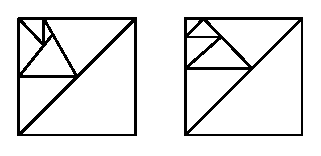
\includegraphics[scale=1.3]{images/chap11/ans16.eps}

\hspace{3cm}\text{7 ತ್ರಿಭುಜಗಳು (ಲಂಬಕೋನ ಸಮದ್ವಿಬಾಹು)}
\end{figure}

\item 
~

\begin{figure}[H]
\centering
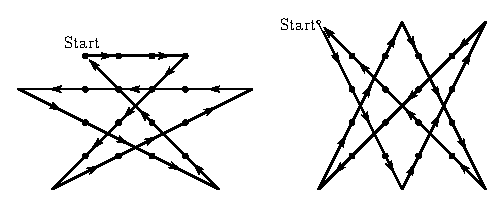
\includegraphics{images/chap11/ans17.eps}
\end{figure}

\item  ಒಟ್ಟು ನವಿಲುಗಳ ಸಂಖ್ಯೆ $x$ ಇರಲಿ. 
{\fontsize{11pt}{13pt}\selectfont
\begin{gather*}
\text{ಸಮೂಹದ}\quad\dfrac{1}{16} ~\text{ ಭಾಗ}~ = \dfrac{x}{16}\\
\text{ಸಮೂಹದ}\quad\dfrac{1}{8} ~\text{ ಭಾಗ}~ = \dfrac{x}{8}\\
\text{ಉಳಿದ ನವಿಲುಗಳು}~ x - \dfrac{x}{16} - \dfrac{x}{8} = \dfrac{13x}{6}\\
\text{ಈ ಸಂಖ್ಯೆಯ}~ \dfrac{1}{3} ~\text{ ಭಾಗ}~ \dfrac{1}{3}\left(\dfrac{13x}{16}\right) = \dfrac{13x}{48}
\end{gather*}

ಇದರ ನಂತರ ಉಳಿದ ಸಂಖ್ಯೆ $\dfrac{13x}{16} - \dfrac{13x}{48} = \dfrac{26x}{48} = \dfrac{13x}{24}$

ಈ ಸಂಖ್ಯೆಯ $\dfrac{1}{6}$ ಭಾಗ  $= \dfrac{1}{6} \left(\dfrac{13x}{24}\right) = \dfrac{13x}{144}$

ಇದಾದ ನಂತರ ಉಳಿದುದು $\dfrac{13x}{24} - \dfrac{13x}{144} = \dfrac{65x}{144}$

ಬಕುಳ ವನದಲ್ಲಿದ್ದ ನವಿಲುಗಳ ಸಂಖ್ಯೆ $\sqrt{x} \times 5$

ಇದನ್ನೂ ಕಳೆದು ಉಳಿದ ನವಿಲುಗಳ ಶೇಷ ಸಂಖ್ಯೆ $\dfrac{65x}{144} - 5\sqrt{x}$

ಇದು 5ಕ್ಕೆ ಸಮ }\relax
\begin{gather*}
\therefore\quad \dfrac{65x}{144} - 5\sqrt{x} = 5\\
65x - 720\sqrt{x} = 720\\
(13x - 144) = 144\sqrt{x}\\
\text{ ವರ್ಗವಣೆ ಮಾಡಿದಾಗ}~ (13x - 144)^{2} = (144\sqrt{x})^{2}\\
169x^{2} - 3744 + 20736 = 20736x\\
169x^{2} - 2448x + 20736 = 0\\
(x - 144)(169x - 144) = 0\\
x = 144 \quad\text{ಅಥವಾ}\quad x = \dfrac{144}{169}
\end{gather*}

ಪೂಣಾಂಕ ಬೆಲೆ ಮಾತ್ರ ಉತ್ತರ $\therefore~ 144$ ನವಿಲುಗಳು 

\item ಎಮ್ಮೆಗಳ ಒಟ್ಟು ಸಂಖ್ಯೆ $x$ ಇರಲಿ 
\begin{gather*}
\left(\dfrac{x}{8} - 1\right)^{2} + 15 = x \quad\text{ ಸಮೀಕರಣ ಲಭಿಸುತ್ತದೆ.}\\
\dfrac{x^{2}}{64} - \dfrac{x}{4} + 1 + 15 = x
\end{gather*}

64 ರಿಂದ ಗುಣಿಸಿದಾಗ 
\begin{align*}
& x^{2} - 16x + 64 + 960 = 64x\\
& x^{2} - 80x + 1024 = 0\\
& (x - 64) (x - 16) = 0
\end{align*}

$\therefore~$ ಎಮ್ಮೆಗಳ ಸಂಖ್ಯೆ 64 ಅಥವಾ  16

\item 
~

\begin{figure}[H]
\centering
\includegraphics[scale=1.1]{images/chap11/ans20.eps}
\end{figure}

$V_{1}$ ಗೋಲದ ಗಾತ್ರ $\dfrac{4}{3} \Pi r^{3}$

$V_{2}$ ಗೋಲದ ಗಾತ್ರ $\dfrac{4}{3} \Pi \left(\dfrac{r}{2}\right)^{3}$
\begin{align*}
\therefore\quad\dfrac{V_{1}}{V_{2}} & = \dfrac{4}{3}\Pi r^{3} \div {\dfrac{4}{3}\Pi \left(\dfrac{r}{2}\right)^{3}}\\
& = \dfrac{\cancel{4}}{\cancel{3}} \cancel{\Pi} \cancel{r^{3}} \times \dfrac{\cancel{3}}{\cancel{4}} \times \dfrac{1}{\cancel{\Pi}} \times \dfrac{2^{2}}{\cancel{r^{3}}} = 2^{3}\\
& = 8
\end{align*}

8 ಸಣ್ಣಗೋಲಗಳನ್ನು ತಯಾರಿಸಬಹುದು. 

\item ಆಯತಾಕಾರದ ಘನದ ಗಾತ್ರ 

$= l\times b\times h = 49\times 44\times 18 = 38808~cm^{3}$

\vskip 0.2cm

ಗೋಲದ ತ್ರಿಜ್ಯ $r$ ಇರಲಿ. ಗಾತ್ರ $\dfrac{4}{3} \Pi r^{3}$

\begin{align*}
\dfrac{4}{3} \Pi r^{3} & = 38808\\
r^{3} & = \dfrac{38808\times 3\times 7}{4\times 22} = 7\times 3\times 441\\
& = 7\times 3\times 7\times 3\times 7\times 3\\
& = 7^{3}\times 3^{3}\\
\therefore\quad r & = 7\times 3 = 21 \text{ ಸೆಂ.ಮೀ.}
\end{align*}

\item 
\begin{tabular}[t]{r}
$8571$\\
$8571$\\
$8571$\\
\hline
$25713$\\
\hline
\end{tabular}

\vskip 0.1cm

ತಪ್ಪು-ಒಪ್ಪು (trial $+$ error) ವಿಧಾನದಿಂದ ಪರಿಹರಿಸಬಹುದು. 

\item 

\begin{tabular}[t]{cccl}
 & 3 ಲೀ ಪಾತ್ರೆ & 5 ಲೀ ಪಾತ್ರೆ & \\
 (1) & $-$ & 5 & (ತುಂಬಿಸಿದೆ)\\
 (2) & 3 & 2 & (5 ರಿಂದ 3 ಲೀ ತುಂಬಿದೆ)\\
 (3) & 0 & 2 & (3 ಲೀ ಖಾಲಿ ಮಾಡಿದೆ)\\
 (4) & 2 & 0 & (2 ಲೀ ನ್ನು 3 ಲೀ ಪಾತ್ರೆಗೆ ಹಾಕಿದೆ)\\
 (5) & 2 & 5 & (5 ಲೀ ಪಾತ್ರೆ ತುಂಬಿದೆ)\\
 (6) & 3 & 4 & (5 ಲೀ ನಿಂದ 3 ಲೀ ಪಾತ್ರೆಗೆ ತುಂಬಿದೆ)
\end{tabular}

\item ಉತ್ತರದ ಅಗತ್ಯವಿಲ್ಲ 

\item ಒಂದು ದಾರದ ಉದ್ದ $x"$ ಇರಲಿ. ಇನ್ನೊಂದು $2x" 6"$ ಕತ್ತರಿಸಿದ ನಂತರ $(x - 6)$, $(2x - 6)$ ಆಗುತ್ತದೆ. 

\begin{align*}
3(x - 6) & = (2x - 6)\\
3x - 18 & = 2x - 6\\
x & = 24\quad\text{ ಮೊದಲ ಅಳತೆ $24"$ಗಳು} 
\end{align*}

\item ಸಂಖ್ಯೆ $x$ ಇರಲಿ. $8x^{2} + 1 = y^{2}$

ತಪ್ಪು-ಒಪ್ಪು ವಿಧಾನದಿಂದ ಪರಿಹರಿಸಿ. $x = 1$ ಆದಾಗ $9$ ಬರುತ್ತದೆ $(9 = 3^{2})$

ಇತರ ಸಂಖ್ಯೆ 6 

\item ಈಗಿನ ವಯಸ್ಸು $x$ ಇರಲಿ 

3 ವರ್ಷದ ನಂತರ $(x+3)$ ಅದರ 3ರಷ್ಟು $3(x+3)$ 

ಮೂರು ವರ್ಷದ ಹಿಂದೆ ವಯಸ್ಸು $(x-3)$ ಅದರ 3ರಷ್ಟು $3(x-3)$
\begin{align*}
3(x + 3) -3(x - 3) & = x\\
3x + 9 - 3x + 9 & = x\\
\therefore\quad x & = 18~\text{ ಈಗಿನ ವಯಸ್ಸು}
\end{align*}

\item ಉತ್ತರದ ಅಗತ್ಯವಿಲ್ಲ 

\item ಉತ್ತರದ ಅಗತ್ಯವಿಲ್ಲ 

\item ಉತ್ತರದ ಅಗತ್ಯವಿಲ್ಲ 
\end{enumerate}
